\documentclass[runningheads,a4paper]{llncs}
%
\usepackage{natbib} % bibliography stuff
%
\usepackage{graphicx} % allows for working with images
\DeclareGraphicsExtensions{.pdf,.png,.jpeg} % configures latex to look for the following image extensions
%
\usepackage{setspace} % allows for configuring the linespacing in the document
%\singlespacing
\onehalfspacing
%\doublespacing
%
\usepackage{amsmath}
%
\usepackage{appendix}
%
\usepackage{multirow}
%
\usepackage{caption}
\captionsetup[table]{skip=10pt}
%
\usepackage[toc]{glossaries}
\makeglossaries
%
\usepackage{amssymb}
\setcounter{tocdepth}{4}
%
\usepackage{url}
\urldef{\mailsa}\path|dkirwan@tssg.org|
\newcommand{\keywords}[1]{\par\addvspace\baselineskip
\noindent\keywordname\enspace\ignorespaces#1}

\begin{document}
\mainmatter  % start of an individual contribution

% first the title is needed
\title{Observing Jovian Decametric Radio Emissions\\
with a Software Defined Radio Telescope}

% a short form should be given in case it is too long for the running head
\titlerunning{Observing Jovian Decametric Radio Emissions}

% the name(s) of the author(s) follow(s) next
%
% NB: Chinese authors should write their first names(s) in front of
% their surnames. This ensures that the names appear correctly in
% the running heads and the author index.
%
\author{David Kirwan%
%\thanks{Please note that the LNCS Editorial assumes that all authors have used
%the western naming convention, with given names preceding surnames. This determines
%the structure of the names in the running heads and the author index.}%
\and Alan Davy\thanks{Supervisors} \and John Ronan\footnotemark[1]}
%
\authorrunning{D. Kirwan}
% (feature abused for this document to repeat the title also on left hand pages)

% the affiliations are given next; don't give your e-mail address
% unless you accept that it will be published
\institute{Waterford Institute of Technology,\\Dept of Maths and Physics,\\
Cork Rd, Waterford City, Ireland\\
\mailsa\\
\url{http://www.wit.ie}}

%
% NB: a more complex sample for affiliations and the mapping to the
% corresponding authors can be found in the file "llncs.dem"
% (search for the string "\mainmatter" where a contribution starts).
% "llncs.dem" accompanies the document class "llncs.cls".
%
\toctitle{Thesis Proposal}
\tocauthor{D. Kirwan}
\maketitle
%
%\begin{abstract}
%The abstract should summarize the contents of the paper and should
%contain at least 70 and at most 150 words. It should be written using %the
%\emph{abstract} environment.
%\keywords{radio astronomy, software defined radio, signal processing}
%\end{abstract}
%
\tableofcontents
%
\newpage
\section*{Introduction}
\addcontentsline{toc}{section}{Introduction}
%This is typically an outline description detailing the background	 to the problem.

\newglossaryentry{DAM}
{
  name={DAM},
  description={decameter radio emissions},
  sort=DAM
}
%
It was discovered in 1954 by \cite{burke55} that the planet Jupiter emits radio transmissions in the decameter (\gls{DAM}) range \textit{10-100 m wavelengths}, and the inner Jovian satellite Io appeared to have an effect on these emissions occurring \citep{belcher87}. Jupiter's radio emissions range between 4 MHz to 39.5 MHZ while emitting most strongly at 8 MHz or so \citep{wilkinson94}. However due to interference from human short wave radio sources between 4-15 MHz coupled with the attenuation of these signals or refraction off Earths ionosphere, the majority of emissions have been observed up in the 15-25 MHz range where this interference is less. The emission signal strength quickly diminishes above this range \citep{wilkinson94}.
%
\begin{figure}[here]
\centering
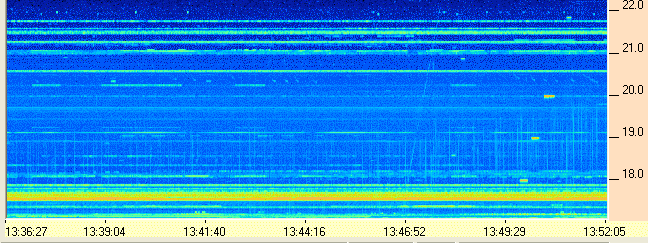
\includegraphics[width=8cm]{images/01}
\caption{Decametric Radio Emissions \citep{ashcraft13}}
\label{fig:dam_Emissions}
\end{figure}
%

Data collected by the two Voyager spacecraft in 1979 \citep{belcher87} and the later Galileo mission in 1995 \citep{kivelson96} added hugely to the understanding of the plasma interactions between Jupiter and Io and the source of the \gls{DAM} emissions. It was discovered that the Io has a thin atmosphere made up of a number of neutral gasses namely sodium, potassium, sulfur, and oxygen as shown in fig: \ref{fig:io_neutral_gasses}. It is generally thought these gasses have been emitted through volcanic activity on the surface of the moon \citep{belcher87}. The gasses in orbit of Io have a very short life time, due to collisions with magnetospheric electrons. This gives rise to a plasma torus (\gls{IPT}) which corotates with Jupiter itself \citep{belcher87}. This can also be seen in fig: \ref{fig:io_neutral_gasses} which shows the \gls{IPT}.
%
\begin{figure}[here]
\centering
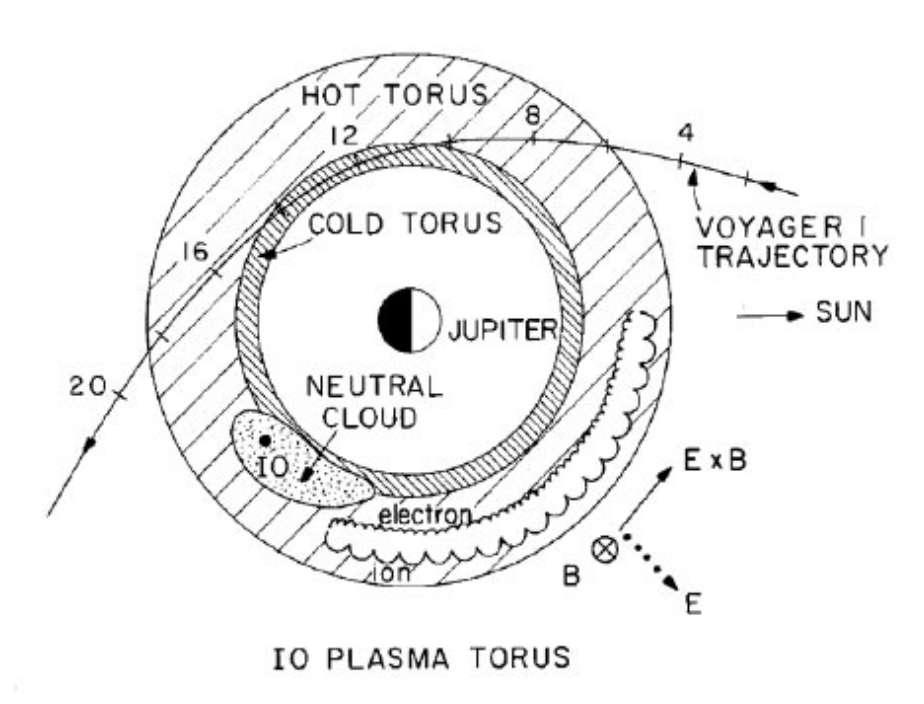
\includegraphics[width=8cm]{images/02}
\caption{Neutral Gasses in Orbit of Io \citep{belcher87}}
\label{fig:io_neutral_gasses}
\end{figure}
%
\newglossaryentry{IPT}
{
  name={IPT},
  description={Io Plasma Torus},
  sort=IPT
}
%

The local corotation speed of the plasma torus is faster than the Keplerian orbit of the moon, and the plasma overtakes Io in its orbit at \begin{math} 57 km\;s^{-1} \end{math} \citep{belcher87}.
%
\newglossaryentry{IFT}
{
  name={IFT},
  description={Io Flux Tube},
  sort=IFT
}
%
Fig \ref{fig:io_flux_tube} details a diagram of the Io Flux Tube (\gls{IFT}) which is a tube made up from Jovian of magnetic field lines \citep{belcher87} which thread the satellite. A large portion of the decametric emissions come from the area where the \gls{IFT} meets the Jovian ionosphere. 
%
\begin{figure}[here]
\centering
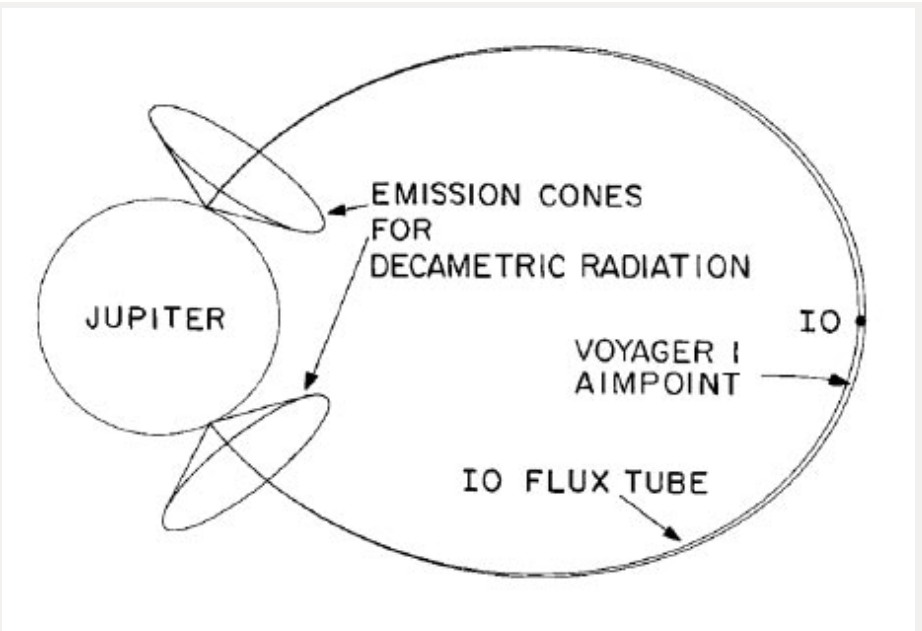
\includegraphics[width=6cm]{images/03}
\caption{Magnetic Flux Tube linking Jupiter and its satellite Io \citep{belcher87}}
\label{fig:io_flux_tube}
\end{figure}
%
As Io orbits within this flux torus it acts as a unipolar conductor \citep{bose08}, and Alfv\'en waves are regularly produced which carry an electric charge along the magnetic field lines between Jupiter and Io \citep{bose08}. These Alfv\'en waves reflect off Jupiters ionosphere at both north and south poles upto 9 times \citep{bose08} while following Io through its orbit, thereby acting as a standing wave. It appears the source of the \gls{DAM} emissions are largely due to these reflections of these Alfv\'en waves off Jupiter's ionosphere.

The \gls{DAM} emissions are carried along the surface of the emission cones as show in fig: \ref{fig:io_flux_tube} \citep{belcher87}. When Io is at specific points in its orbit of Jupiter, emissions are released at the surface of this cone. When pointing in Earths direction, it can be picked up at ground based radio telescope listening stations.

%
\begin{figure}[here]
\centering
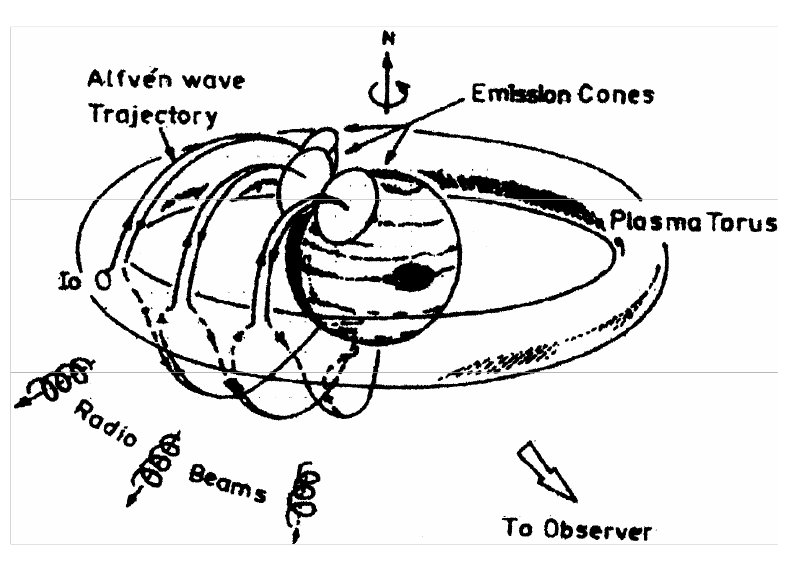
\includegraphics[width=8cm]{images/04}
\caption{DAM Emissions from Jupiter \citep{bose08}}
\label{fig:io_flux_tube}
\end{figure}
%

%
%%%%%%%%%%%%%%%%%%%%%%%%%%%%%%%%%%%%%%%%%%%%%%%%%%%%%%%%%%%%%%%%%%%%%%%%%%%%%%%%%%%%%%%%%%%
%
\newpage
\section*{Research Topic}
\addcontentsline{toc}{section}{Research Topic}
%Students should identify whether the research outcomes are likely to have universal application or have a defined scope. This is important in gauging the extent to which the work is capable of independent replication.
%
%
\newglossaryentry{WRC}
{
  name={WRC},
  description={World Radiocommunication Conference},
  sort=WRC
}
\newglossaryentry{HF}
{
  name={HF},
  description={High Frequency},
  sort=HF
}
%
A ground based listening station aiming to record \gls{DAM} emissions from Jupiter is most likely to succeed between 15-25 MHz \citep{wilkinson94}. The \textit{shortwave radio} bands extend from 2.3 MHz (120 m) all the way to 26.1 MHz (11 m) and were approved for broadcast at the 1997 World Radio communication Conference (\gls{WRC}). ComReg, is the Irish Commission for Communications Regulation within Ireland, and maintains a list of the short wave frequencies which are designated for transmission in Ireland and can be seen in fig: \ref{fig:irish_electromagnetic_transmission_ranges} \citep{comreg14}.

%
\begin{figure}[here]
\centering
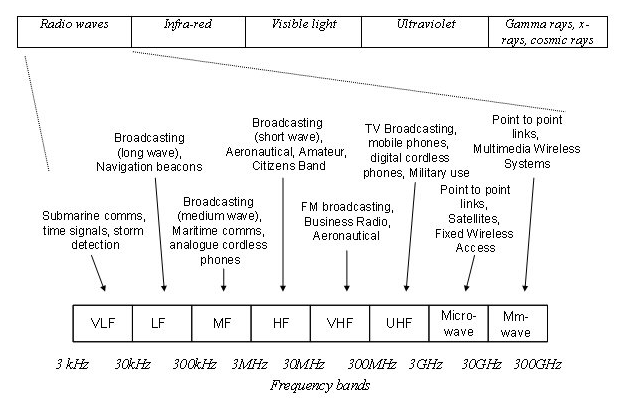
\includegraphics[width=8cm]{images/06}
\caption{Irish Regulatory Transmission Ranges \citep{comreg14}}
\label{fig:irish_electromagnetic_transmission_ranges}
\end{figure}
%

As many commercial shortwave radio stations transmit in the lower end of the high frequency (\gls{HF}) 3-7 MHz range, it can be extremely busy and potentially difficult to monitor \gls{DAM} emissions where they are strongest. Amateur radio operators also operate frequently in mid-late \gls{HF} ranges while the higher frequency \gls{DAM} emissions taper off in strength very quickly. This limits the potential listening range significantly. Despite these obstacles, there are sections of the \gls{HF} spectrum which are suitable to capture Jovian emissions. The a suitable frequency to monitor Jovian \gls{DAM} emissions which is recommended by the Radio Jove project is \textit{20.1 MHz} \citep{nasa12}. 

Sourcing a suitable antenna is one of the first requirements to satisfy in order to capture \gls{DAM} emissions. Antennas generally are best suited to collect electromagnetic radiation at single specific frequencies, but may resonate and therefore operate over a range of frequencies depending on the design \citep{nasa12}. The wavelength ($\lambda$) which corresponds with the frequency (\textit{f}) \textit{20.1 MHz} can be obtained using the wavelength equation as shown in fig \ref{fig:wavelength_equation}. The corresponding wavelength for the frequency \textit{20.1 MHz} works out to be \textit{14.925 m} using this equation.

%
\begin{figure}[here]
  \centering
  \begin{equation}  	
    \lambda = \frac{c}{f}
  \end{equation}
  \begin{equation}
    \lambda = \frac{3x10^8 m/s}{20.1x10^6 Hz} = 14.925373134328359 m
  \end{equation}
  \caption{Wavelength Equation}
  \label{fig:wavelength_equation}
\end{figure}
%

One simple antenna design for collecting \gls{DAM} emissions is the \textit{dipole}. A dipole antenna can be constructed simply and cheaply from two pieces of wire and three insulators \citep{nasa12}, while ensuring to cut the wires to a length matching half the desired wavelength being captured \citep{nasa12}. However as the formula referenced in fig: \ref{fig:wavelength_equation} describes the use of an \textit{infinitely thin} wire which is not possible in reality, \textit{capacitive end effects} must be taken into account when working out the resonating wavelength for a dipole antenna \citep{nasa12}.

The formula for calculating the resonating frequency for a half wavelength dipole is described in fig \ref{fig:wavelength_equation_dipole} and produces the value which should measure from tip to tip on the wires used to construct the dipole antenna \citep{nasa12}.

%
\begin{figure}[here]
  \centering
  \begin{equation}  	
    \bigg(\frac{\lambda}{2}\bigg)m = \frac{142.65}{20.1 MHz} = 7.097014925373134 m
  \end{equation}
  \caption{Wavelength Equation for Real World Half Wavelength Dipole Antenna}
  \label{fig:wavelength_equation_dipole}
\end{figure}
%

The radio emissions come in several different forms each with slightly different characteristics. Table: \ref{tab:dam_emissions} shows a list of the more widely known types which can be picked up using ground based listening equipment, and also has some information about their different characteristics \citep{wilkinson94}. Any particular observation session might be made up of some or all of these different types of \gls{DAM} emission and can last from a few minutes to several hours for larger noise storms \citep{wilkinson94}.

%
\begin{table}
  \centering
  \begin{tabular}[pos]{| c | c | c |}
    \hline
    Type & Emission Length & Emission Description\\ \hline
    S-Bursts & short generally 1-10 milliseconds & wideband bursts, several MHz wide\\ \hline
    L-Bursts & long 0.5 - 5 seconds & wideband bursts, several MHz wide\\ \hline
    N-Bursts & milliseconds upto seconds & narrowband bursts, several kHz wide\\
    \hline
  \end{tabular}
  \caption{Most common types of DAM Emissions from Jupiter \citep{wilkinson94}}
  \label{tab:dam_emissions}
\end{table}
%

Fig: \ref{fig:dam_emissions_spectrum} shows an ideal case of the \textit{S-Burst} and \textit{L-Burst} \gls{DAM} emissions and what they might look like on a frequency spectrum graph. S-Burst emissions are short, generally $1-10x10^{-3}s$ long while L-Bursts can be \textit{0.5-5s} in length.

%
\begin{figure}[here]
\centering
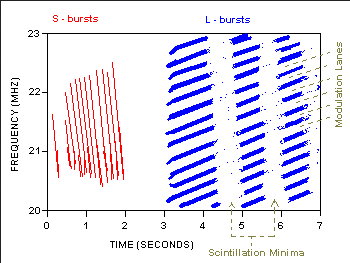
\includegraphics[width=8cm]{images/05}
\caption{Ideal DAM Emissions types from Jupiter \citep{wilkinson94}}
\label{fig:dam_emissions_spectrum}
\end{figure}
%
%%%%%%%%%%%%%%%%%%%%%%%%%%%%%%%%%%%%%%%%%%%%%%%%%%%%%%%%%%%%%%%%%%%%%%%%%%%%%%%%%%%%%%%%%%%
%
\newpage
\section*{Research Problem}
\addcontentsline{toc}{section}{Research Problem}
%
\newglossaryentry{SDR}
{
  name={SDR},
  description={Software Defined Radio},
  sort=SDR
}

The aim of this project is to design and construct a low cost, self sufficient software defined radio (\gls{SDR}) telescope listening station, which can capture signals for transmission to a central data aggregation point for signal processing and analysis. This telescope should be suitable to study signals  in the \gls{DAM} (10-100 m) band at or near the \textit{20.1 MHz} frequency in order to pick up emissions produced by either Jupiter or the Sun.

There are a number of challenges which need to be overcome to achieve this, such as Jupiter only being visible for a number of months each year and then generally in the evening, night, or morning hours. Often at highly unsociable times. For this reason a radio telescope listening site should be as automated as possible.

%
\begin{figure}[here]
\centering
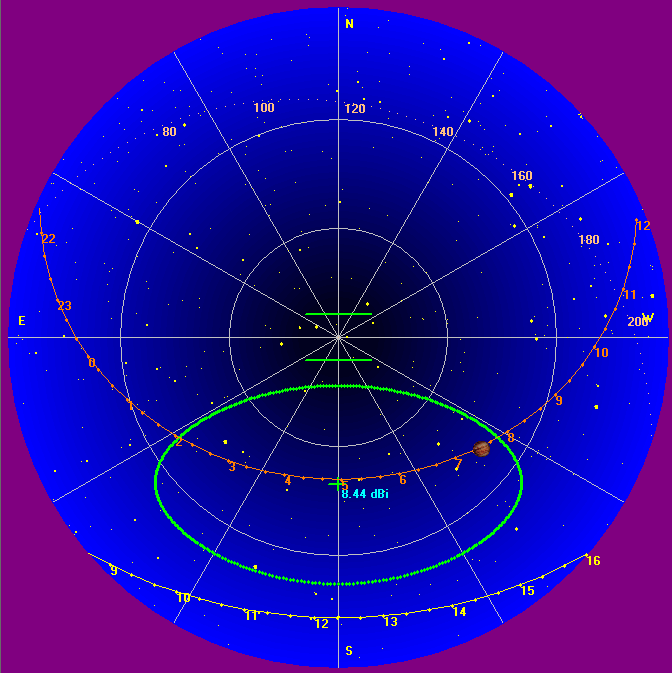
\includegraphics[width=8cm]{images/07}
\caption{Dual Dipole Antenna Beam at 20FT and 135deg phasing S \citep{nasa12}}
\label{fig:dual_dipole_20ft_135phasing_s}
\end{figure}
%

During daylight hours, the ionosphere becomes opaque to signals in the \gls{DAM} band due to becoming ionised by solar radiation \citep{nasa-ionosphere-12}. The proposed system will have a short window in the order of 1-6 hours every second night and early morning or so during which it may be possible to capture \gls{DAM} emissions from Jupiter. The Sun is a source of \gls{DAM} emissions also, and the telescope can capture solar storm emissions without modification, providing the Sun passes through the antenna beam. The telescope may require manual reconfiguration in order to pick up solar storm emissions during the day.


%
\begin{figure}[here]
\centering
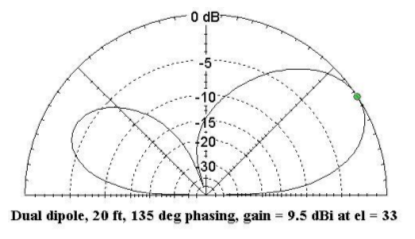
\includegraphics[width=8cm]{images/09}
\caption{Dual Dipole Antenna Array Beam\citep{nasa12}}
\label{fig:dual_dipole_antenna_array_beam}
\end{figure}
%


Interference from human sources such as shortwave radio stations or amateur radio operators are also likely to affect the collection of \gls{DAM} emissions from Jupiter. The ability for automated flagging or removal of interference would be a desirable feature of the system. Lightning storms can also produce interference which will affect observations, it might be desirable for the system to handle natural interference sources also.

%
\begin{figure}[here]
\centering
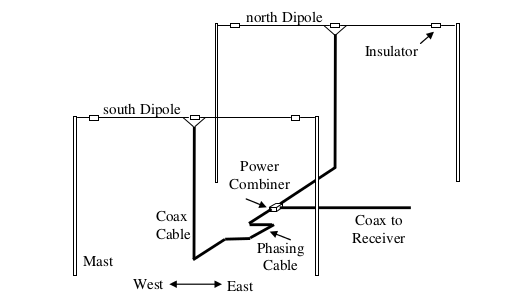
\includegraphics[width=8cm]{images/08}
\caption{Dual Dipole Antenna Array \citep{nasa12}}
\label{fig:dual_dipole_antenna_array}
\end{figure}
%

\subsection*{Problem Summary}
\addcontentsline{toc}{subsection}{Problem Summary}

To summarise the problem briefly:

\begin{itemize}
  \item Design of a low cost self sufficient SDR telescope platform suitable for amateur observers
  \item Capable of studying Jupiter in the decametric band 3MHz - 40MHz (10-100 m)
  \item This band is chosen because Earths atmosphere is transparent at these frequencies during the night time
  \item Another reason is emissions near 20Mhz, are least likely to be interfered with from human short wave sources
  \item Such a platform has a second capability in that it is also be capable of studying Solar emissions during the day as solar emissions are strong enough to penetrate the ionosphere during the day
  \item Development of a backhaul system for processing and storage of listening site captured data, thereby making it capable of aggregating data from multiple listening sites
  \item Develop an API for accessing this data, and allow integrating into 3rd party applications
  \item Amateur listening sites can compliment larger telescope arrays around the world
\end{itemize}


%
%%%%%%%%%%%%%%%%%%%%%%%%%%%%%%%%%%%%%%%%%%%%%%%%%%%%%%%%%%%%%%%%%%%%%%%%%%%%%%%%%%%%%%%%%%%
%
\section*{Research Questions}
\addcontentsline{toc}{section}{Research Questions}
%A clear, precise definition of the problem is very important to focus on the research activity. great care should be used in devising the research questions. They define the structure of the investigation/innovation that will be used and an essential metric of the quality of the dissertation is the degree to which the research question has/have been answered.
The initial research questions which arise are as follows:

\newglossaryentry{IOT}
{
  name={IOT},
  description={Internet of Things},
  sort=IOT
}

\begin{itemize}
  \item What current Internet of Things (\gls{IOT}) technologies would best suit the development of a fully automated software defined radio signal listening station and how cheaply can it be created?
  \item Can a software defined radio solution be developed to filter or flag known instances of human radio interference from radio signal observations?
  \item If so can this same solution be used to filter or flag known instances of natural radio interference such as lightning?
\end{itemize}


%
%%%%%%%%%%%%%%%%%%%%%%%%%%%%%%%%%%%%%%%%%%%%%%%%%%%%%%%%%%%%%%%%%%%%%%%%%%%%%%%%%%%%%%%%%%%
%
\newpage
\section*{Research Hypothesis}
\addcontentsline{toc}{section}{Research Hypothesis}
%This should outline the approach and methodology being proposed by the student to address the research question.

The section aims to document the different methodologies which will be followed on this project and is broke up into the following:


\begin{description}
  \item[Antenna Build] \hfill \\
    Building the antenna is further broken down into the following steps:
    \begin{itemize}
      \item source materials to build a dual dipole antenna
      \item build the telescope antenna
      \item validate the antenna is capable of collecting signals at or near the 20.1 MHz frequency \\
    \end{itemize}
  \item [Analysis of Listening Site Suitability] \hfill \\
    Finding a site suitable to deploy the antenna will require a site survey with the antenna connected to a spectrum analyser.
    \begin{itemize}
      \item source a spectrum analyser suitable for performing a site survey
      \item perform the survey at this site
      \item repeat until suitable site is found 
      \item deploy the antenna at a site \\
    \end{itemize}
  \item [Data Collection] \hfill \\
    Jupiter is visible above the horizon at night only during certain periods see fig: \ref{fig:dual_dipole_antenna_array_beam}. In order to perform the required data collection it is highly desirable to automate the process.
    \begin{itemize}
      \item create listening schedule during which \gls{DAM} emissions are likely to occur
      \item develop \gls{SDR} prototype mechanism for gathering raw data from the antenna
      \item develop software scheduling system which to activate the collection of data from the antenna remotely\\
    \end{itemize}
  \item [Data Analysis] \hfill \\
    Collected data can be analysed manually at first in order to validate the testbed, but later using software such as the development of basic algorithms to spot events such as \textit{S-Bursts} occurring in the data.
    \begin{itemize}
      \item analyse data collected for evidence of Jovian or Solar \gls{DAM} emissions
      \item analyse data for evidence of interference from human sources
      \item analyse data for evidence of interference from natural sources
      \item develop a system which connects to the dxspider server and creates flag events for human identified emissions at or near the target frequency being monitored by the telescope
      \item develop a system which interacts with the Blitzortung servers and creates flag events for emissions generated by lightning \\
    \end{itemize}
  \item [Data Processing] \hfill \\
    \gls{SDR} data processing techniques can be developed in order to better filter the signals as they are being collected thereby minimising the level of processing at a later stage.
    \begin{itemize}
      \item using \gls{SDR} techniques, to reduce interference in data as it is being collected
      \item attempt to remove instances of human and natural interference using signal processing techniques after collection \\
    \end{itemize}
  \item [Data Aggregation] \hfill \\
    An API layer allows 3rd parties the ability to access data collected from multiple listening sites and potentially develop new features or systems using the data.
    \begin{itemize}
      \item develop API layer to allow external parties access aggregated data collected by the system \\
    \end{itemize}
  \item [Design Platform] \hfill \\
    An analysis of the current available \gls{IOT} technologies and some of the available options which could be used in order to produce an open low cost platform which amateur astronomers could use in order to study emissions in the \gls{DAM} band.
    \begin{itemize}
      \item design a self sufficient automated platform suitable for collection of signals such as those by the \gls{SDR} telescope \\
    \end{itemize}
\end{description}

The \gls{SDR} hardware transceiver used is likely to be the \textit{HackRF} system while the \gls{SDR} software components will be developed in either \textit{C++} or \textit{Python} as both languages have bindings for the \textit{GNURadio} development toolkit \citep{gnuradio-14}. The backend aggregation system with API will most likely be developed in the \textit{Ruby} language as this language is highly expressive and suitable for rapid prototype development. Execution of the Ruby application on the Java VM is capable using the \textit{JRuby} system, which will also allow the incorporation of any required Java libraries.


\subsection*{Potential Pitfalls}
\addcontentsline{toc}{subsection}{Potential Pitfalls}
%Predecisions on how I want to collect data, creating the research questions

It is difficult to determine at this early stage what will ultimately prove to be the most troublesome element to implement, however there are a number of potential pitfalls which have already been identified.

%
\begin{figure}[here]
\centering
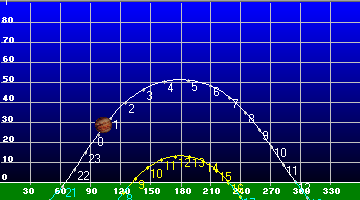
\includegraphics[width=8cm]{images/11}
\caption{Radio Jove Graph Showing Jupiters Max Altitude 2014}
\label{fig:jupiter_max_altitude_2014}
\end{figure}
%

The latitude of Ireland is 53.3$^{\circ}$ degrees N. In Ireland Jupiter reaches a maximum altitude of 52$^{\circ}$ degrees in 2014 see fig: \ref{fig:jupiter_max_altitude_2014}. The telescope configuration which will be documented will apply only to locations at this or a similar latitude. It will be universally applicable at this latitude without modification throughout the world, and with relatively minor modifications to the configuration of the antenna it can be used at all locations. \cite{nasa12}

The \gls{SDR} complexity of the solution required in order to correctly filter interference might ultimately prove too resource intensive to work with a low power system such as the \textit{Raspberry Pi} or \textit{Beaglebone Black}. It might become apparent that the minimum system requirements may need to be increased to an \textit{Intel Atom} powered Netbook for example, or potentially something a lot more powerful such as an \textit{i3} or \textit{i5} system. If this was the case, it will drastically increase the power and cost requirements of the system should it be self sufficient, requiring bigger batteries, more capable/expensive photovoltaic and or wind turbines to keep the system topped up.

%
%%%%%%%%%%%%%%%%%%%%%%%%%%%%%%%%%%%%%%%%%%%%%%%%%%%%%%%%%%%%%%%%%%%%%%%%%%%%%%%%%%%%%%%%%%%
%
\newpage
\section*{Preliminary Literature Review}
\addcontentsline{toc}{section}{Preliminary Literature Review}
%This should contain a review of a number of books, journal articles and web references of relevance to the research area proposed. The literature should contain seminal and recent referenced research material that is categorised under a number of relevant sub-themes.

%WIP:

I've read about 15 papers already related to the background of the interactions between Jupiter and Io, and papers detailing results from similar telescopes to the design I intend to build. I've hit a paywall on some of the earliest seminal papers which were the first to detail the phenomenon of decametric emissions being emitted by the Jupiter-Io system. I will attempt to get a copy through the inter library loan system at WIT.


My literature review can be broken down into the following areas:

\begin{itemize}
  \item What are the decametric radio emissions and what are they caused by
  \item Research journals detailing potential radio telescope designs which could be replicated in order to collect DAM emissions
  \item I need to look into journals involving signal processing and maybe some rudimentary filtering or AI for identifying spurious signals
  \item Something else
  
\end{itemize}
%
%%%%%%%%%%%%%%%%%%%%%%%%%%%%%%%%%%%%%%%%%%%%%%%%%%%%%%%%%%%%%%%%%%%%%%%%%%%%%%%%%%%%%%%%%%%
%
\newpage
\section*{Contribution to Research Knowledge Anticipated}
\addcontentsline{toc}{section}{Contribution to Research Knowledge Anticipated}
%
A dissertation is a work of scholarly investigation that is grounded in the research literature and differs from a report or a book. It is judged on a prescribed set of academic criteria. Although the likely outcomes are tentative at hte start of the program, it is useful to incorporate them into the research proposal to help focus the work program.
%
%%%%%%%%%%%%%%%%%%%%%%%%%%%%%%%%%%%%%%%%%%%%%%%%%%%%%%%%%%%%%%%%%%%%%%%%%%%%%%%%%%%%%%%%%%%
%
\newpage
\section*{Description of the Experimental Design / Validation Methodology}
\addcontentsline{toc}{section}{Description of the Experimental Design / Validation Methodology}
%
A dissertation must employ rigorous scientific argument. The experimental design and the validation methodology must be specified in great detail in the proposal. At this proposal stage you should define clear evaluation criteria.


\begin{itemize}
  \item Identify data caused by lightning
  \item Identify data caused by human emissions
  \item Perform a site survey with the spectrum analyser
  \item Replicate the testbed at a second site
\end{itemize}
%
%%%%%%%%%%%%%%%%%%%%%%%%%%%%%%%%%%%%%%%%%%%%%%%%%%%%%%%%%%%%%%%%%%%%%%%%%%%%%%%%%%%%%%%%%%%
%
\newpage
\section*{Special Resources Required}
\addcontentsline{toc}{section}{Special Resources Required}
%
The research work may require access to specialised equipment, software, journals and so on.

Access to the HackRF or another similar SDR is required.
Access to the RadioJove Prediction software
%
%%%%%%%%%%%%%%%%%%%%%%%%%%%%%%%%%%%%%%%%%%%%%%%%%%%%%%%%%%%%%%%%%%%%%%%%%%%%%%%%%%%%%%%%%%%
%
\newpage
\section*{Main Milestones Anticipated}
\addcontentsline{toc}{section}{Main Milestones Anticipated}
%
Students should agree a number of milestones and their likely delivery dates with their supervisor at the start of the progress.


\begin{itemize}
  \item Design the testbed
  \item Build the telescope
  \item Perform a site survey with the spectrum analyser
  \item Replicate the testbed at a second site
\end{itemize}


%
\printglossaries
%
\newpage
\listoftables
\addcontentsline{toc}{chapter}{List of Tables}
%
\bibliographystyle{plainnat}
\bibliography{bibliography/bibtex}
\addcontentsline{toc}{chapter}{Bibliography}
%
\newpage
%
\appendix
\section*{Appendix}
\addcontentsline{toc}{chapter}{Appendices}
Here is some content in the appendix

\begin{subappendices}
\subsection*{How I became inspired}
Lorem ipsum dolor sit amet, consectetur adipiscing elit. Praesent ut egestas sapien. Sed vehicula, libero vitae ornare interdum, nunc felis rhoncus risus, ut lobortis quam ligula sed nunc. Suspendisse potenti. Proin lacinia ex dui, eu maximus justo consequat porttitor. Pellentesque sollicitudin rutrum ex hendrerit vestibulum. Etiam luctus leo vitae magna sagittis feugiat a vitae ligula. Maecenas suscipit interdum tincidunt. Etiam a sapien elit. Nam dictum sed felis non commodo.

%
\end{subappendices}

\end{document}


